
\textbf{Produção de Lote Pioneiro de Sensor Inteligente:}

Foram apresentados sensores de voltagem e corrente para linhas de transmissão
que podem tanto ser alimentados pela rede secundária 220V ou por painel solar
(100mW) caso esta não esteja disponível. Cada sensor consome 14mW e se comunica
por GPRS, onde seus dados são exibidos em um software com indicação para cada
local instalado.
A instalação de cada sensor consome entorno de 40min. A análise do impacto do
primeiro lote no tempo de resposta da operadora da rede em caso de avarias na
rede se mostrou muito mais curto, com reduções de até 1h ou 2h,
figura~\ref{fig::bebado}.

\begin{figure}[h!]	
	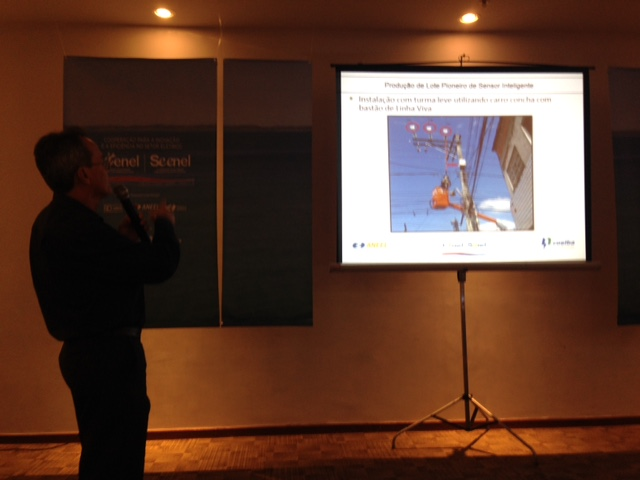
\includegraphics[width=\columnwidth]{figs/bebado.JPG}
	\caption{Ilustração da palestra Produção de Lote Pioneiro de Sensor Inteligente}
	\label{fig::bebado}
\end{figure}